%% -----------------------------------------------------------------------------

\chapter{Design and Implementation}\label{ch:design}
\glsresetall % Resets all acronyms to not used
\glsunset{IEEE} \glsunset{MAC}

This chapter proposes a method of detecting \gls{MAC} addresses through sample correlation. The algorithm is implemented in Matlab as a proof-of-concept.


%% -----------------------------------------------------------------------------

\section{High-Level Sender Detector Design}

The high-level design of a sender detector based on \gls{MAC} addresses is illustrated in Figure \ref{fig:blockdesign}. From the beginning of my work until the final version, multiple design choices have changed. These and their reasons are depicted in detail in Chapter 5. The overall concept has however remained unmodified.

\begin{figure}[H]
	\centering
	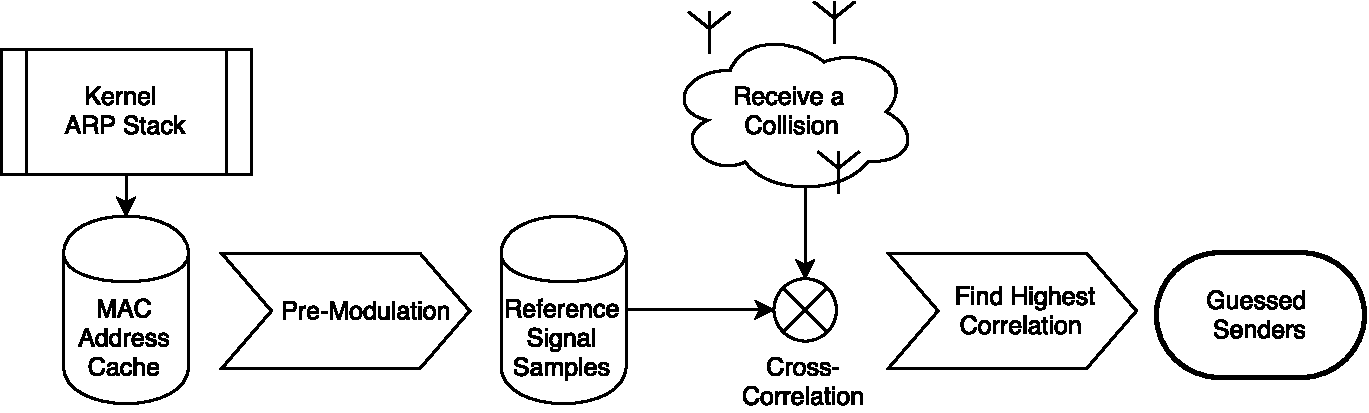
\includegraphics[width=\textwidth]{gfx/images/detector-block-design}
	\caption[High-Level Detector Design Schema]{High-Level Detector Design Schema}
	\label{fig:blockdesign}
\end{figure}

First of all, it is important to decide which \gls{MAC} addresses should be tested when processing a received collision. Since \gls{MAC} addresses are six byte values, there are $2^{48} \approx 3 \cdot 10^{14}$ possible instances. Although some \gls{MAC} addresses are invalid because the first three bytes denote the network interface vendor, and not all values have been issued\footnote{http://standards-oui.ieee.org/oui.txt}, there are still by far too many to try out all of them for every collision.

Instead, I make use of the operating system's \gls{ARP} stack. During normal network operation, the kernel already keeps a cache of \gls{MAC} addresses that have been observed. This list is perfectly suited for detecting senders, as it is quite likely that a collision occurs between senders that are already in the network for some time.\\

Next, I modulate IEEE 802.11 data frames for every cached \gls{MAC} address. These are used as reference signals for correlation with incoming collisions. Only a small chunk of the reference frames contains the \gls{MAC} address bits and is thus important for sender detection. I describe this region in detail in section \ref{sec:mac-periods}.

As mentioned in section \ref{sec:mac-and-phy}, there are different possibilities for frame encoding, namely the \gls{MCS}, the scrambler initialization, and the error-correcting convolutional encoding. Since the convolutional encoder uses a seven bit state, only the \gls{MAC} header field directly preceding the sender \gls{MAC} address is relevant here. That field is the destination \gls{MAC} address. In theory, all possible combinations could be modulated for the reference signals cache, however this would mean a total amount of  more than 130 thousand candidates for every \gls{MAC} address in the ARP pool. I evaluate the impact of these factors in chapter \ref{ch:evaluation}.

The amount of 130 thousand candidates, as mentioned above, is the product of three values: $ N_{\text{MCS}} $ denotes the possible Modulation and Coding Schemes, which are eight. $ N_{\text{Scrambler}} $ describes the available scrambler initialization values. For a seven bit state where the value zero is invalid \cite{ieee2012}, these are $ 2^7 - 1 = 127 $. $ N_{\text{Dest}} $ is the amount of possible states of the convolutional encoder, which are $ 2^7 = 128 $.

$$ N_{\text{MCS}} \cdot N_{\text{Scrambler}} \cdot N_{\text{Dest}} = 8 \cdot 127 \cdot 128 = 130 048 $$\vspace{0cm}

The modulation process comprises the following steps:

\begin{enumerate}
	\item Generate a \gls{MAC} header with appropriate sender and destination \gls{MAC} addresses
	\item Apply the scrambler with specific initialization value
	\item Run the convolutional encoder, which is deterministic
	\item Group bits and interleave symbols
	\item For a time-domain signal, apply \gls{IFFT} and add a cyclic prefix
\end{enumerate}

For correlation in the frequency domain, I omit step five. The \gls{FFT} has to be applied to the received collision signal in this case. I have done experiments with frequency-domain detection and show the results of these in section \ref{sec:freqd-correlation}.\\

When the receiver senses a transmission, I determine whether it is a collision using the IEEE 802.11 \gls{LTF}. Section \ref{sec:preamble-corr} gives details about this process. This also measures a possible delay between the two frames.

Upon noticing a collision, all reference samples are correlated with the signal under test. The correlations are then sorted in descending order by correlation magnitude. The highest correlations make up for the best guess which senders are subject to the collision.\\

It is worth noting that the output of this algorithm is always a probabilistic result. The technique will never detect senders with full confidence, but rather return a distribution of likelihood over the cache of reasonable \gls{MAC} addresses.


%% -----------------------------------------------------------------------------

\section{Detecting Frames and Collisions}\label{sec:preamble-corr}

A receiver captures a continuous stream of samples, generated by its \gls{ADC}. It is necessary to employ some mechanism to detect the start of a transmission. In regular operation, IEEE 802.11 receivers use the known preamble for this by correlating the \gls{LTF} to the incoming data in a sliding window approach \cite{perahia2013}.

This can be extended to recognizing collisions. Since the \gls{LTF} is designed in a way that it has low off-peak autocorrelation \cite{ieee2012}, there will be twice as many correlation peaks in a collision of two frames. The distance between the two \gls{LTF} pattern can even be used to calculate a possible delay between the two transmissions. An example of such correlation peaks in case of a collision is shown in Figure \ref{fig:preamble-corr}. Each frame causes two large spikes, and one spike with smaller magnitude. This is caused by the composition of the \gls{LTF} with two repetitions of a symbol, and a cyclic prefix of half the symbol size.\\

Knowing when the frames start is important for sender detection. Since the \gls{MAC} address is represented by only a small number of time-domain samples (see section \ref{sec:mac-periods}), it is vital to correlate the correct chunk of the signal.

\begin{figure}[H]
	\centering
	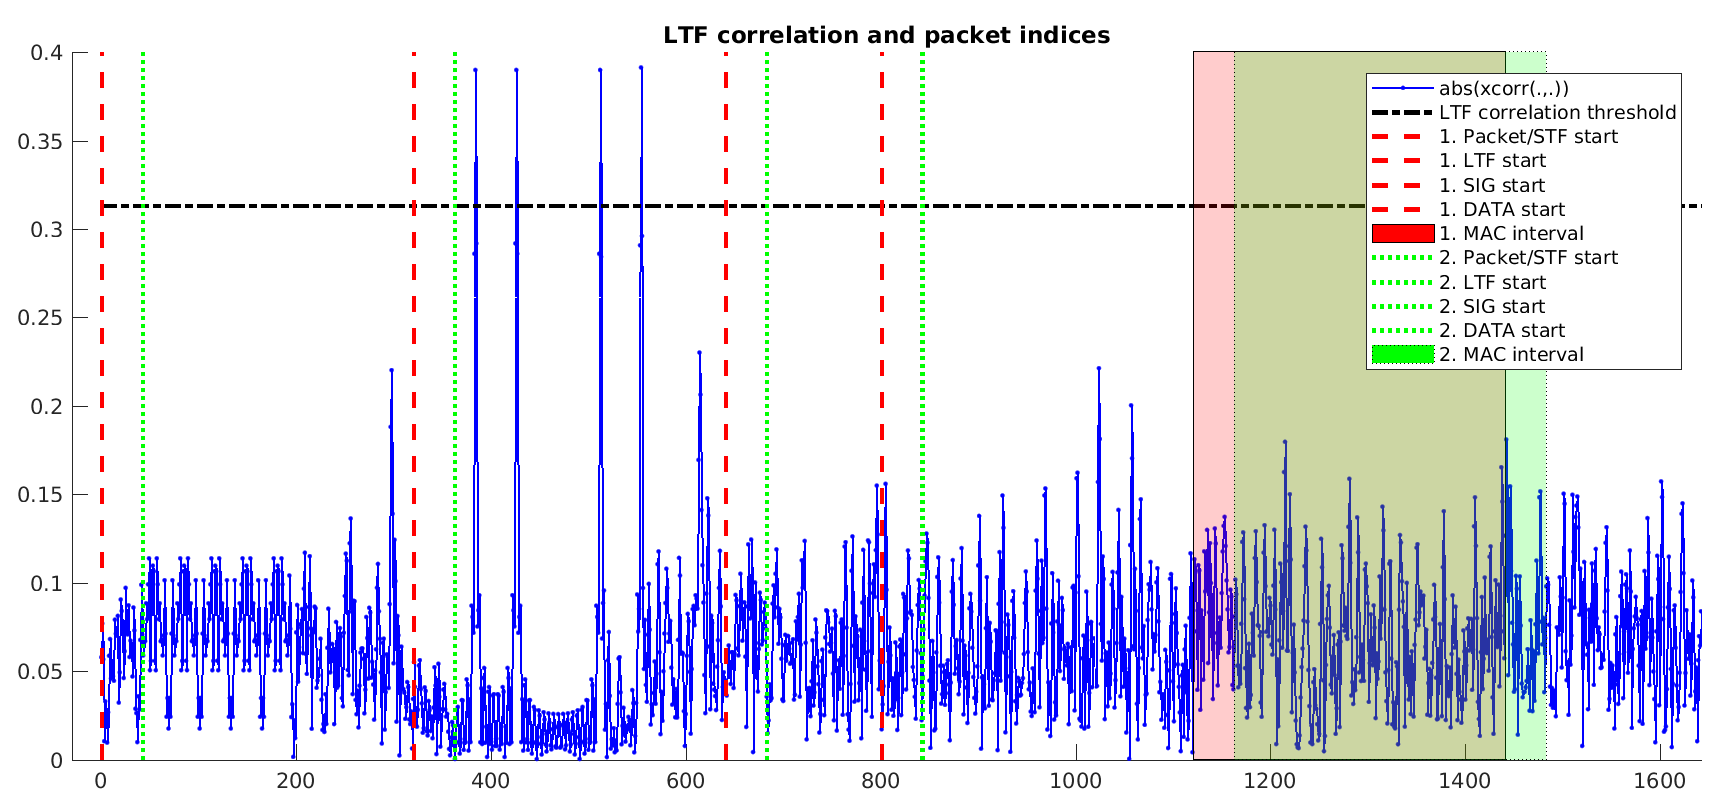
\includegraphics[width=\textwidth]{gfx/plots/preamble}
	\caption{Cross Correlation of Collision Samples with Long Training Field}
	\label{fig:preamble-corr}
\end{figure}

Figure \ref{fig:preamble-corr} offers additional markers for the different signal fields as described in section \ref{sec:mac-and-phy}. Here, the symbols containing the \gls{MAC} address of the first frame begin after 1120 samples. The second \gls{MAC} address follows with an offset of about 40 samples.

When trying to decode these \gls{MAC} addresses, the correlations with the reference pool signals obviously have to be applied to the combined region of the first and second \gls{MAC} addresses. In this example, that would be all of the colored samples.


%% -----------------------------------------------------------------------------

\section{Periods Containing MAC Addresses}\label{sec:mac-periods}

Depending on the \gls{MCS}, the samples affected by different \gls{MAC} addresses start at different positions. The byte offset within the \gls{MAC} layer header remains the same. However, the amount of \gls{OFDM} symbols that need to be skipped before the beginning of the \gls{MAC} address, and the symbol count that has to be included to cover everything, change depending on the bit density.

Table \ref{tbl:sample-offsets} provides a summary of the various samples offsets for different \glspl{MCS}. These values are calculated assuming a sampling rate of 20 MHz. Since IEEE 802.11a/g channels have a passband bandwidth of 20 MHz, this is the minimum required sampling rate \cite{ieee2012}. However, some radios like the \gls{WARP} boards use a higher sampling rate of 40 MHz. In this case, all indices have to be doubled.\\

All frames begin with the preamble, specifically the Short and Long Training Fields, and the Signal Field. Both the \gls{STF} and \gls{LTF} have a duration of 8 $\mu$s. For the \gls{STF}, this is 10 repetitions of a 0.8 $\mu$s symbol. For the \gls{LTF}, there are two repetitions of a 3.2 $\mu$s symbol, and the 1.6 $\mu$s cyclic prefix. The Signal Field consists of one standard \gls{OFDM} symbol with cyclic prefix. That is 4 $\mu$s in the case of IEEE 802.11.

In total, the preamble takes 20 $\mu$s. At 20 MHz sampling rate, this results in $ 20 \cdot 10^{-6} s \cdot 20 \cdot 10^6 Hz= 400 $ samples. The Data Field thus start at sample index 401. Within that, the Service Field as well as the Frame Control and Duration \gls{MAC} header fields precede the \gls{MAC} addresses.\\

\begin{table}[ht]
	\centering
	\begin{tabular}{|p{2.5cm}|p{4.5cm}|p{4.5cm}|}
		\hline
		\textbf{MCS} & \textbf{Address 1 (Destination)} & \textbf{Address 2 (Sender)} \\ \hline
		0 & 561 - 720 & 721 - 880 \\ \hline
		1 & 481 - 640 & 561 - 720 \\ \hline
		2 & 481 - 560 & 561 - 640 \\ \hline
		3 & 401 - 560 & 481 - 560 \\ \hline
		4 & 401 - 480 & 481 - 560 \\ \hline
		5 & 401 - 480 & 401 - 480 \\ \hline
		6 & 401 - 480 & 401 - 480 \\ \hline
		7 & 401 - 480 & 401 - 480 \\ \hline
	\end{tabular}
	\caption{Sample Offsets of MAC Address Fields at Different MCSs}
	\label{tbl:sample-offsets}
\end{table}

\glspl{MCS} 0 and 2 have an important advantage. Only with these schemes does the above described region contain only the specific \gls{MAC} address, since the encoded bits per \gls{OFDM} symbol (24 for \gls{MCS} 0, and 48 for \gls{MCS} 1, as mentioned in Table \ref{tbl:mcs}) are integer multiples of the 48 bits \gls{MAC} address length. All other schemes contain additional data before the address, behind it, or in both positions.


%% -----------------------------------------------------------------------------

\section{Matlab Implementation}\label{sec:matlab-impl}

I built a proof of concept implementation of the presented technique in Matlab. Matlab was initially chosen for its large number of suitable toolboxes, and an existing implementation of the 802.11 MAC and PHY. It also allows to use \gls{WARP} \glspl{SDR}. The WARPLab 7.5.1 Matlab \gls{SDK}\footnote{http://warpproject.org/trac/wiki/WARPLab} provides easy-to-use high-level access to the radios. It was my preferred choice over the alternative of using Python and \gls{USRP} boards.\\

The Matlab code is structured into different sections. First, utility functions implement the generation of \gls{MAC} headers, modulating IEEE 802.11 data frames in the time domain, and choosing sender \gls{MAC} addresses randomly from a list. There are two different libraries used for modulation: MathWorks' WLAN System Toolbox\footnote{https://www.mathworks.com/products/wlan-system.html} as well as a custom IEEE 802.11 implementation developed at the \gls{SEEMOO} at TU Darmstadt.

A number of simulation scripts measure the detection algorithm's performance under simulated channel effects. The results of these are presented in chapter \ref{ch:evaluation}. A WARPLab script effectively does the same thing, but using three \gls{WARP} \glspl{SDR}. Finally, there are scripts that run a series of experiments varying certain parameters, save the data, and generate figures for evaluation.\\

The core of the Matlab implementation is cross-correlation. Using the Signal Processing Toolbox\footnote{https://www.mathworks.com/products/signal.html}, this can be done using the \texttt{xcorr} function. This function expects two complex sample series and returns a complex correlation vector and a real vector of offsets. The offsets range from the negative feature length up to the positive length. This is because the data series can be slided against each other in both directions. Using this function is similar to this example for an \gls{LTF} symbol:\\

\begin{lstlisting}[captionpos=b,caption={Cross-Correlation of an LTF Symbol},label=lst:xcorr]
[correlation, offset] = xcorr(rx, lts_t);
\end{lstlisting}

Analyzing the performance of my implementation revealed that most time was not spent on cross-correlation, but on the generation of the reference signal pool. I improved this code by applying the following optimizations.

First, since the sender detection only relies on correlating those samples that contain the \gls{MAC} address, as described in section \ref{sec:mac-periods}, most of the generated signal is discarded anyways. This means that it is unnecessary to spend valuable time on calculating the \gls{MAC} layer checksum, which is stored after the payload data. I simple use a placeholder value of 0x42424242 for the checksum. Furthermore, I do not generate the preamble, namely the Training and Signal Fields. This can be done by using the \texttt{wlanNonHTData} function from the WLAN System Toolbox. This function merely modulates the Data Field, in contrast to the \texttt{wlanWaveformGenerator} function.

Second, I store the reference signals in a cache that is reused in as many consecutive experiments as possible. All experiments were repeated for at least 100 runs. Since the reference pool remained the same for all repetitions, using a shared variable for the entire set almost cut the cost of a higher sample size to zero. This is because in relation to modulating a signal, calculating cross-correlations consumes several orders of magnitude less time (about 0.2 ms compared to 650 ms). This is good news because in a real-world application, the generation of reference signals can be done ahead of time, and signals under test do not have to be modulated since they are received already in the time domain.

Incorporating these optimizations reduced the runtime of the experiment varying the scrambler initialization, which is presented in section \ref{sec:ex-scrambler}, from an extrapolated 300 days to about 45 minutes on a consumer laptop. This not only allowed me to run the experiments at all, but also let me increase the number of repetitions, and therefore largely enhancing the sample size.\\

To simulate channel effects, different channel models from both the WLAN System Toolbox and the Communications System Toolbox \footnote{https://www.mathworks.com/products/communications.html} were used. The exact functions are described in the corresponding sections in chapter \ref{ch:evaluation}.\\

As addressed in section \ref{sec:preamble-corr}, it is necessary to detect the offset between two frames in a collision. This is done using the \texttt{meshgrid} Matlab function. Listing \ref{lst:meshgrid} shows an example of calculating the field indices of both collided frames. The code compares the signal-to-training symbol correlation with a defined threshold and finds peaks in the data. These are then grouped into four clusters. This effectively removes noise and measuring inaccuracies causing a spike to last for more than one sample. Due to the correlation of the preamble with one \gls{LTF} symbol, there should be two large and one small spike. This is because as described in section \ref{sec:mac-and-phy}, the \gls{LTF} comprises two symbol repetitions and a cyclic prefix of half a symbol length. Since the correlation threshold is chosen to be between the small and large spike, and assuming that exactly two frames collided, the expected amount of peaks is therefore four.

\begin{lstlisting}[captionpos=b,caption={Collision Offset Detection using Meshgrid},label=lst:meshgrid]
% Find peaks above a parametrized threshold
lts_peaks = find(abs(correlation) > LTS_CORR_THRESHOLD*max(abs(correlation)));

% Assuming two frames, there will be four high peaks
[~, C] = kmeans(lts_peaks', 4);
uniq_lts_peaks = sort(floor(C))';

% Select the best candidate correlation peak at LTS-payload boundary
[LTS1, LTS2] = meshgrid(uniq_lts_peaks, uniq_lts_peaks);
[lts_second_peak_index, y] = find(iswithin( ...
    LTS2-LTS1, ...
    length(lts_t)/1.2, ...
    length(lts_t)*1.2 ...
));

% Add 128 samples for the symbol itself (at 40 MHz)
ind2.sig = uniq_lts_peaks(max(lts_second_peak_index)) + 128;
ind2.ltf = ind2.sig - 320; % subtract LTF length
ind2.stf = ind2.ltf - 320; % subtract STF length
ind2.payload = ind2.sig + 160; % add 4us SIG field
ind1.sig = uniq_lts_peaks(min(lts_second_peak_index)) + 128;
ind1.ltf = ind1.sig - 320;
ind1.stf = ind1.ltf - 320;
ind1.payload = ind1.sig + 160;
\end{lstlisting}

The \texttt{meshgrid} function then calculates a two-dimensional table of all possible offsets between every two peaks. Using the \texttt{find} function, I look for offsets that equal the length of one training symbol with a 20 percent margin. This margin makes the algorithm a bit more reliable against slight timing imprecision. The offset between the collided frames is the delay between these symbol matches.

Lastly, the signal field sample indices are calculated as the last symbol's correlation peak plus the length of that symbol, which is 128 samples at 40 MHz sampling rate. Start indices of the \gls{LTF}, \gls{STF}, and Data Field are deduced accordingly.\\

The indices are stored in a structure, which is later used to cut out the samples containing the sender's MAC address. That set is determined as the start of the address in the first frame until the end of the address in the second frame. Especially on real hardware, this allows to mitigate possible delays and offset between the frames.
